\documentclass[10pt,conference]{IEEEtran}

\usepackage[T1]{fontenc}
\usepackage{cite}
\usepackage{graphicx}
\usepackage{booktabs}
\usepackage{tabularx}
\usepackage{array}
\usepackage{xcolor}
\usepackage{xurl}
\usepackage{enumitem}
\usepackage[hidelinks]{hyperref}

\newcolumntype{Y}{>{\raggedright\arraybackslash}X}
\newcolumntype{L}[1]{>{\raggedright\arraybackslash}p{#1}}
\setlist[itemize]{leftmargin=*, itemsep=1pt, topsep=2pt}
\setlist[enumerate]{leftmargin=*, itemsep=1pt, topsep=2pt}

\title{Humans Were the Bug: From Vibe Coding to Agent-Native Engineering}
\author{\IEEEauthorblockN{humanlint Project}}

\begin{document}

\begin{titlepage}
\centering
\vspace*{0.15in}
{\LARGE\bfseries Humans Were the Bug: From Vibe Coding to Agent-Native Engineering\par}
\vspace{0.6em}
{\normalsize humanlint Project\par}
\vspace{1.0em}
\IfFileExists{assets/humanlint_header.png}{%
  
\includegraphics[width=0.91\textwidth,height=0.40\textheight,keepaspectratio]{assets/humanlint_header.png}%
}{%
  
\includegraphics[width=0.91\textwidth,height=0.40\textheight,keepaspectratio]{../assets/humanlint_header.png}%
}
\vspace{1.1em}

\begin{minipage}{0.92\textwidth}
\begin{abstract}
AI coding changes the primary failure mode of software organizations. The bottleneck is no longer whether a human knows a language well enough to type plausible code; modern agents can produce plausible Rust, Go, TypeScript, Python, SQL, and shell in the same session. The bottleneck is whether the repository can reject wrong generated code quickly, localize the defect, prove the repair, preserve security posture, and teach the next agent what happened.

This paper argues that codebases optimized for human memory, taste, and informal review are now misaligned with agentic maintenance. It proposes an agent-native standard centered on a narrow winning stack: Rust core, TypeScript/React/Vite product surface, PostgreSQL durable truth, generated contracts, and bounded Python for AI/data service work. The stack is not chosen because it is most pleasant to write. It is chosen because it gives the strongest combined surface for compile-time rejection, contract enforcement, database truth, deterministic testing, security audit, observability, and repair routing.

The contribution is operational: a 100-point stack rubric, a top-five stack ranking, a winner-only architecture, an agent-first repository standard, an exception design pattern, a test coverage model, and a CI audit rubric for detecting vibe-coding behavior. The audit treats dead-language markers such as ``legacy,'' ``deprecated,'' ``temporary,'' ``fallback,'' ``stub,'' and ``TODO'' as repair signals unless explicitly justified as product copy or documented exceptions. The end state is not human-free engineering. It is human-directed engineering where repositories become verification interfaces for agents.
\end{abstract}

\begin{IEEEkeywords}
AI-assisted software engineering, agentic coding, repository architecture, Rust, TypeScript, PostgreSQL, software audit, verification, code generation.
\end{IEEEkeywords}
\end{minipage}
\vfill
\end{titlepage}

\section{Introduction}

The title is intentionally blunt, but the claim is narrower than the insult. Humans were not the bug because humans wrote software. Humans were the bug because most repositories were shaped around human memory, human patience, human stylistic preference, and slow human review. That design worked only while code arrived slowly enough for teams to compensate through taste, folklore, and senior-engineer recall. Agentic coding removes that throttle.

GitHub's 2025 Octoverse report describes an ecosystem where AI is already mainstream in development and where TypeScript has become the most-used language on GitHub \cite{githubOctoverse2025}. DORA's 2025 research frames AI as an amplifier of existing organizational capability rather than an automatic productivity guarantee \cite{doraStateAIAssistedSoftwareDevelopment2025}. Security evidence is harsher: Veracode reports that generated code can be syntactically plausible while still containing known flaws \cite{veracodeGenaiCodeSecurity2025}, and GitGuardian reports accelerating secret exposure in public GitHub activity, including AI-assisted commits \cite{gitguardianSecretsSprawl2026,gitguardianSecretsSprawl2026Blog}. The correct response is not to slow agents down until the old process survives. The correct response is to redesign the codebase as the control surface that constrains, proves, and repairs agent work.

This paper makes four claims. First, programming languages should be understood as compression technologies for human and organizational bottlenecks. Second, once agents can learn syntax on demand, language choice shifts from author comfort toward rejection speed, security, proof locality, and auditability. Third, the strongest general-purpose target stack is Rust core plus TypeScript/React/Vite plus PostgreSQL plus generated contracts plus bounded Python. Fourth, the winning stack matters only if repositories enforce it through layout, tests, generated zones, exceptions, documentation, and CI audit.

\section{Languages as Compression Technology}

Programming language history is often told as a progression toward abstraction. That is incomplete. A language is a compression package: it decides which burdens move from human memory into syntax, type systems, runtimes, libraries, tooling, and conventions. Machine code compressed nothing. Assembly compressed opcodes into names. Fortran compressed scientific arithmetic. COBOL compressed business records. C compressed portable systems programming into a thin abstraction over hardware. Java compressed memory management and deployment portability into a managed runtime. Python compressed exploration and glue. JavaScript compressed browser programmability. TypeScript compressed large-team JavaScript maintenance by adding a static feedback loop to the browser ecosystem, a direction now strengthened by Microsoft's native TypeScript 7 effort \cite{typescript70Beta2026}.

\begin{table*}[t]
\caption{Language evolution as bottleneck compression rather than linear progress.}
\label{tab:language-history}
\centering
\small
\begin{tabularx}{\textwidth}{L{0.20\textwidth} Y Y}
\toprule
\textbf{Era or family} & \textbf{Human bottleneck compressed} & \textbf{Agent-era interpretation} \\
\midrule
Machine code and assembly & Remembering opcodes, addresses, registers, and jumps. & Exactness without reviewability is not enough; agent patches need semantic structure. \\
Fortran and COBOL & Expressing domain work without writing every machine operation. & Domain vocabulary matters because agents need stable concepts to route changes. \\
C and Unix systems programming & Portable control over hardware, memory, and operating-system interfaces. & Power without structural memory safety increases audit burden; CISA/NSA guidance pushes teams toward memory-safe defaults \cite{cisaMemorySafeLanguages2025}. \\
Java and .NET & Managed memory, deployment portability, enterprise libraries, and tooling. & Mature ecosystems are valuable, but framework surface can hide ownership boundaries. \\
Python, R, Julia & Exploration, data analysis, notebooks, and scientific productivity. & Excellent for model/data loops; dangerous when unbounded into product truth. Python 3.14 improves runtime options, but does not change the boundary problem \cite{python314Release2025}. \\
JavaScript and TypeScript & Browser programming, product velocity, and typed frontend maintenance. & Essential product surface; should not become durable backend truth. \\
Rust and modern safe systems languages & Memory safety, ownership, concurrency discipline, and explicit error handling. & Strong core for agent-generated code because invalid states can be rejected before runtime. \\
\bottomrule
\end{tabularx}
\end{table*}

The agent-era lesson is that syntax is no longer the scarce resource. A model can imitate syntax. It cannot reliably infer unstated ownership, hidden exception policies, or tribal boundaries. The language and repository must make the invalid path structurally harder.

\subsection{Why Languages Fracture}

New languages emerge when an existing compression package stops matching the dominant pain. They fracture around runtime ceilings, ecosystem gaps, tooling weakness, migration cost, hiring constraints, interop friction, and fashion that lacks enforcement. A language can be technically excellent and still fail as a default company architecture if it lacks the operational surround: boring deployment, security scanning, observability, package maturity, database migration norms, and enough public examples for agents and humans to learn from.

Julia is the cleanest example of legitimate promise without universal adoption. Its multiple dispatch, JIT compilation, and scientific-computing focus attack the two-language problem in numerical work: prototype in a high-level language, then rewrite hot paths in C, C++, or Fortran \cite{bezansonJulia2017}. That is a real problem and Julia remains a serious answer for many scientific domains. The adoption lesson is not that Julia is bad. The lesson is that solving an inner-loop expression problem does not automatically solve company-scale product engineering, cloud operations, security review, hiring, packaging, and cross-language contract discipline.

\begin{table*}[t]
\caption{Dead-hype and niche-language shelf: serious promise, constrained adoption.}
\label{tab:dead-hype}
\centering
\small
\begin{tabularx}{\textwidth}{L{0.15\textwidth} Y Y Y}
\toprule
\textbf{Language or ecosystem} & \textbf{Real promise} & \textbf{Adoption limiter} & \textbf{Agent-era penalty} \\
\midrule
Julia & Scientific productivity with performance-oriented multiple dispatch. & Broader product engineering ecosystem and deployment defaults lag dominant stacks. & Thinner general-product corpus and more local conventions. \\
D & Better C++-class systems language ergonomics. & Could not displace entrenched C/C++ ecosystems and tooling gravity. & Smaller examples and weaker enterprise defaults. \\
Nim and Crystal & Python/Ruby-like ergonomics with native compilation. & Smaller communities, fewer boring production patterns. & Agents get fewer canonical examples and fewer tool-enforced boundaries. \\
Elm & Frontend reliability and no-runtime-exception ambition. & Ecosystem and interop constraints limited broad adoption. & Excellent lessons, but narrow hiring/corpus surface. \\
Reason/OCaml frontend & Typed functional UI with serious compiler roots. & Tooling and community fragmentation. & Harder for general agents to infer local conventions. \\
F\# and Clojure & High-leverage functional design on mature runtimes. & Strong niches, smaller mainstream product footprint. & Expert-friendly abstractions can become opaque to repair agents. \\
Haskell and Scala & Powerful type-system and abstraction research translated to production niches. & Complexity and hiring/training friction. & Proof power helps only when conventions are explicit and common. \\
Elixir/Phoenix & Fault tolerance, supervision, realtime systems on the BEAM. & Specialist fit rather than universal product default. & Wins realtime collaboration, not general stack standardization. \\
\bottomrule
\end{tabularx}
\end{table*}

The shelf is not a graveyard of bad ideas. It is evidence that technical elegance and universal default status are different things. Agent-native engineering rewards stacks where examples, tools, contracts, tests, and deployment conventions are abundant enough that agents can be constrained rather than merely prompted.

\section{The Harsh AI Reality}

AI assistance makes second place more expensive. In the pre-agent era, a language that was pleasant to humans could win locally because human familiarity was the bottleneck. In the agent era, familiarity is weaker as a deciding variable. Agents can produce plausible code in most mainstream languages; the differentiator becomes how quickly the system rejects false plausibility.

That change should make teams more severe, not more permissive. DORA's amplifier finding means weak review, weak tests, weak architecture, and weak platform engineering will be amplified \cite{doraStateAIAssistedSoftwareDevelopment2025}. Veracode's GenAI security results mean syntax success does not imply security success \cite{veracodeGenaiCodeSecurity2025}. GitGuardian's secret-sprawl evidence means AI-churned repositories need stronger secret gates, not more trust \cite{gitguardianSecretsSprawl2026}. The winning organization will not be the team with the friendliest prompt. It will be the team whose repository turns generated code into a bounded hypothesis and then proves, rejects, or repairs it.

\section{Method: A 100-Point Stack Rubric}

The rubric below scores a stack for durable product systems maintained by agents and humans together. It deliberately weights correctness, security, contracts, and repairability above product velocity because AI already lowers the cost of first drafts. The scarce resource is trustworthy merge.

\begin{table*}[t]
\caption{humanlint 100-point stack rubric for agent-native product engineering.}
\label{tab:stack-rubric}
\centering
\small
\begin{tabularx}{\textwidth}{L{0.21\textwidth} L{0.07\textwidth} Y Y}
\toprule
\textbf{Criterion} & \textbf{Weight} & \textbf{Full-credit signal} & \textbf{Evidence and argument} \\
\midrule
Agent-verifiable correctness loop & 18 & Fast type/compile checks, deterministic test routing, generated contracts, property tests, reproducible local and CI lanes. & AI output must be treated as suspect until a proof loop rejects or accepts it; setup and context benchmarks show environment and retrieval reliability are central bottlenecks \cite{setupBench2025,contextBench2026}. \\
Security, memory safety, supply chain & 16 & Memory-safe core, secret scanning, SCA, SBOM/provenance, lockfiles, unsafe ledger, dependency rationale. & CISA/NSA memory-safety guidance, Veracode GenAI findings, and GitGuardian secrets evidence all push security into structural gates \cite{cisaMemorySafeLanguages2025,veracodeGenaiCodeSecurity2025,gitguardianSecretsSprawl2026}. \\
Runtime performance, memory, cloud cost & 13 & Efficient hot path, predictable latency, bounded memory, cheap concurrency, low cold-start cost. & Agent-era systems are compute-heavy and parallel; runtime cost becomes architectural, not cosmetic. \\
Concurrency and resilience & 12 & Structured async, cancellation, backpressure, idempotency, retries, dead-letter handling, replayable workflows. & Go survey evidence shows broad AI use but persistent quality concerns; concurrency needs guardrails rather than cleverness \cite{goDeveloperSurvey2025}. \\
Boundary and contract integrity & 11 & OpenAPI/Protobuf/JSON Schema sources, generated clients, schema drift checks, migration gates. & Cross-language systems work only when contracts are generated and tested; OpenAPI Generator and Buf provide mature paths \cite{openapiGeneratorUsage2026,bufDocs2026}. \\
Simplicity and review surface & 10 & Small files, narrow modules, explicit ownership, boring dependency direction, low duplication. & Agents over-edit when boundaries are implicit; SWE-agent and SWE-bench show interfaces and environment shape affect agent results \cite{sweAgentAci2024,sweBench2024}. \\
Ecosystem, hiring, AI corpus strength & 8 & Large corpus, maintained packages, common deployment patterns, strong model familiarity. & GitHub Octoverse language patterns and TypeScript's rise matter because public examples are part of the agent substrate \cite{githubOctoverse2025}. \\
Observability, auditability, provenance & 6 & OpenTelemetry traces/metrics/logs, request IDs, release provenance, repair receipts. & OpenTelemetry gives a vendor-neutral vocabulary for post-merge repair \cite{openTelemetryDocs2025,otelSemanticConventions2026}. \\
Data integrity and durable workflow fit & 4 & PostgreSQL constraints, migrations, indexes, RLS where useful, transactional workflow safety. & PostgreSQL constraints and row-security policies move durable truth below fallible application code \cite{postgresConstraints2026,postgresRowSecurity2026}. \\
Product velocity and interop & 2 & Fast UI loop, generated clients, easy local dev, standard browser ecosystem. & TypeScript 7 and Vite 8 improve feedback speed, but velocity is deliberately weighted below proof \cite{typescript70Beta2026,vite80Release2026}. \\
\bottomrule
\end{tabularx}
\end{table*}

Points are awarded only for structural properties. ``We review carefully'' is not a security control. ``The senior engineer knows where SQL belongs'' is not a boundary. ``The README explains it'' is not a generated contract. The stack must make the wrong path hard to express and the right path cheap to prove.

\section{Top-Five Stack Ranking}

\begin{table}[t]
\caption{Top-five stack results under the humanlint rubric.}
\label{tab:stack-ranking}
\centering
\small
\begin{tabularx}{\columnwidth}{L{0.10\columnwidth} Y L{0.13\columnwidth}}
\toprule
\textbf{Rank} & \textbf{Stack} & \textbf{Score} \\
\midrule
1 & Rust core + TypeScript/React/Vite + PostgreSQL & 94 \\
2 & Go services + TypeScript/React/Vite + PostgreSQL & 90 \\
3 & C\#/.NET + TypeScript/React/Vite + PostgreSQL/SQL Server & 89 \\
4 & TypeScript product plane + Rust/Go compute cells + PostgreSQL & 88 \\
5 & Kotlin/Java JVM + TypeScript/React/Vite + PostgreSQL/Kafka & 87 \\
\bottomrule
\end{tabularx}
\end{table}

\begin{figure*}[t]
\centering
\IfFileExists{paper/figures/stack-ranking.pdf}{%
  
\includegraphics[width=0.88\textwidth]{paper/figures/stack-ranking.pdf}%
}{%
  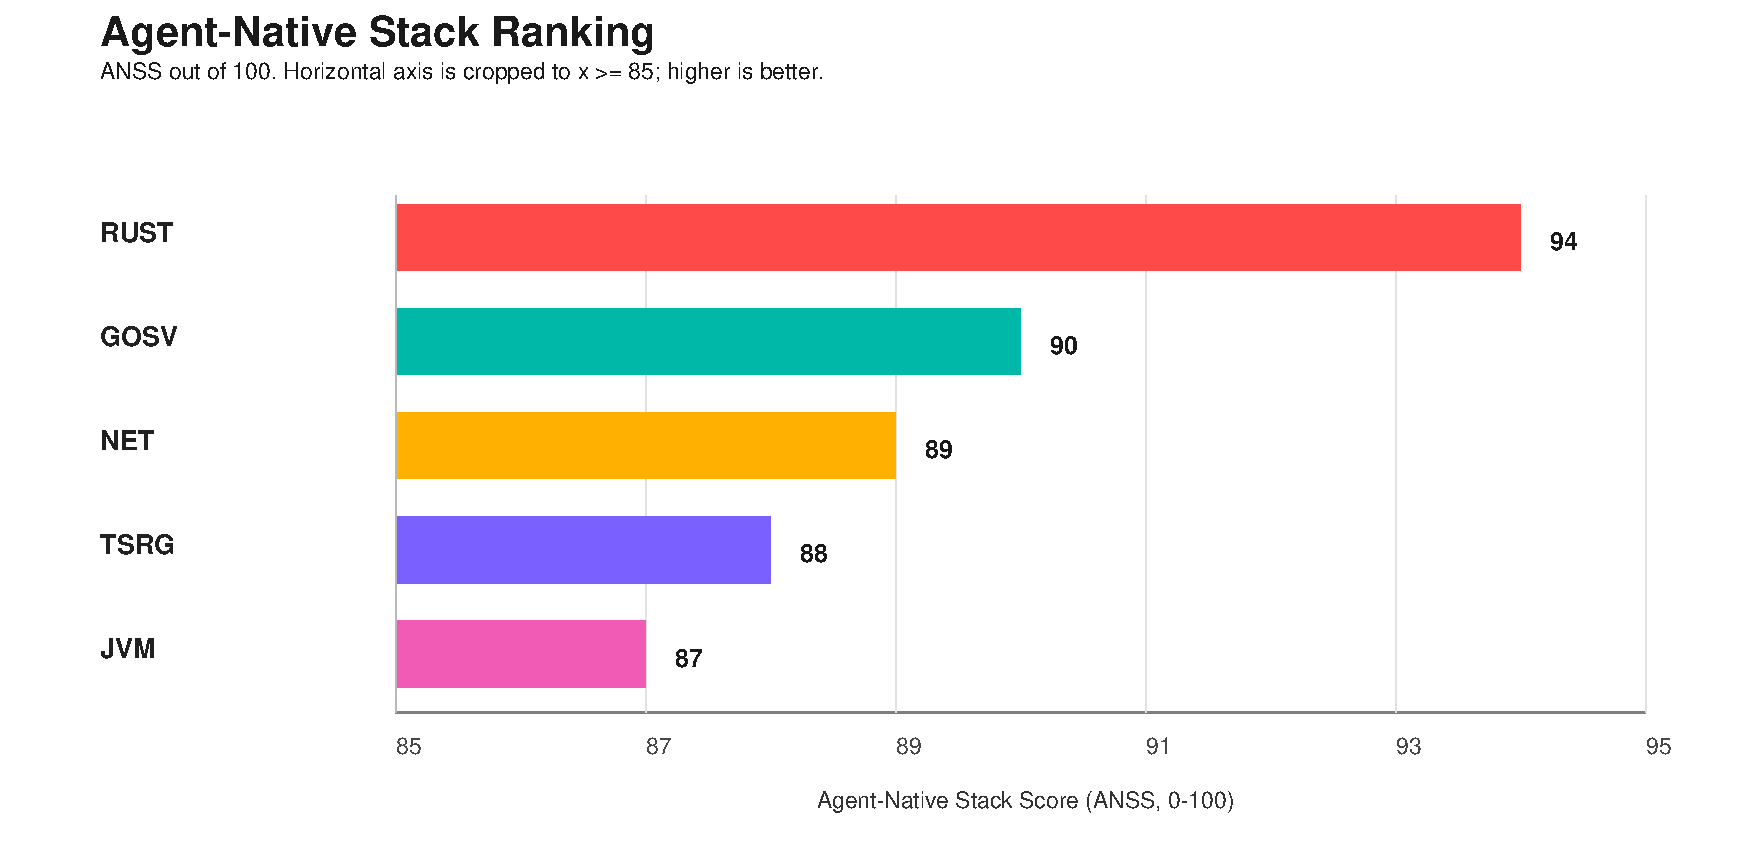
\includegraphics[width=0.88\textwidth]{figures/stack-ranking.pdf}%
}
\caption{Top-five stack ranking. The x-axis minimum is 80\% of the lowest score, so the plotted range starts at 69.6.}
\label{fig:stack-ranking}
\end{figure*}

The small gap between ranks two through five is real. Go is the best practical default for many companies: simple, fast, cloud-native, and easy to standardize. .NET is the strongest enterprise/regulatory answer where Microsoft platform fit is part of proof speed. A TypeScript-heavy product plane with Rust or Go compute cells can be the fastest product-velocity compromise. Kotlin/Java remains powerful where JVM and mobile ecosystems dominate. Elixir/Phoenix deserves a specialist override for realtime collaboration, presence, and fault-tolerant coordination.

The standard, however, should optimize for the winner. The target architecture is Rust core, TypeScript/React/Vite product surface, PostgreSQL truth, generated contracts, and bounded Python AI/data service. Rust wins the core because memory safety, ownership, enums, privacy, exhaustive matching, and explicit error handling let teams encode decisions that other stacks leave to review discipline. TypeScript wins the product surface because the browser and AI corpus are there, and TypeScript/Vite are becoming faster feedback loops \cite{githubOctoverse2025,typescript70Beta2026,vite80Release2026}. PostgreSQL wins durable truth because constraints, transactions, indexes, and row security can reject application mistakes below the code layer \cite{postgresConstraints2026,postgresRowSecurity2026}. Python stays because AI/data work lives there, but it must be boxed.

\section{Winner-Only Architecture}

Once a standard identifies the target, continuing to optimize for every runner-up becomes noise. The agent needs one default map. The audit needs one default policy. CI needs one default set of gates.

\begin{table*}[t]
\caption{Default ownership cells for the winning stack.}
\label{tab:ownership}
\centering
\small
\begin{tabularx}{\textwidth}{L{0.18\textwidth} Y Y}
\toprule
\textbf{Cell} & \textbf{Owns} & \textbf{Must not own} \\
\midrule
\texttt{apps/web} & React UI, route state, forms, local validation, generated API clients, Playwright tests. & Secrets, durable truth, direct SQL, core authorization, handwritten API mirrors. \\
\texttt{apps/api} & Rust HTTP/RPC edge, request normalization, auth middleware, idempotency keys, response shaping. & Domain invariants hidden in handlers, scattered SQL, UI concerns. \\
\texttt{domain} crate & IDs, value objects, invariants, state machines, pure decisions, stable error types. & I/O, env reads, network, filesystem, database clients, framework code. \\
\texttt{application} crate & Commands, authz, transaction orchestration, idempotency, workflow use cases. & Transport details, SQL drivers, UI state, prompt/model logic. \\
\texttt{adapters} crate & PostgreSQL access, queues, external APIs, filesystem, environment, provider clients. & Domain rules. \\
\texttt{workers} crate & Async jobs, retries, backoff, workflow replay, scheduled tasks. & Duplicated invariants or unowned product truth. \\
\texttt{contracts} & OpenAPI, Protobuf, JSON Schema, generated stubs and clients. & Hand-edited generated outputs or business logic. \\
\texttt{db} & Migrations, constraints, indexes, RLS, seed rules, schema snapshots. & Application orchestration or hidden business process. \\
\texttt{python/ai-service} & Inference, embeddings, evals, prompt experiments, offline transforms, typed AI API. & Product truth, authz, billing, direct production DB ownership. \\
\texttt{ops} & CI, release, telemetry, secret scanning, SBOM/SCA, provenance, policy gates. & Feature behavior hidden behind manual operations. \\
\bottomrule
\end{tabularx}
\end{table*}

The filesystem should be a routing table. A patch touching a payment invariant should land in Rust domain/application and PostgreSQL constraints. A patch touching a form should land in TypeScript UI and generated client contracts. A patch touching model behavior should land in the bounded Python service and contract tests. If the agent must infer ownership from convention, the repo has already failed.

\section{Agent-First Repository Design}

Public agent tooling converges on one lesson: instructions matter, but deterministic control surfaces matter more. Codex supports project guidance through \texttt{AGENTS.md} \cite{openaiCodexAgentsMd2026}. The community \texttt{AGENTS.md} specification frames the file as a plain Markdown companion for coding agents \cite{agentsMdSpec2026}. Claude Code loads project memory through \texttt{CLAUDE.md} and related hierarchy \cite{claudeCodeMemoryDocs2026}. Cursor uses project rules with scope metadata \cite{cursorRulesDocs2026}. GitHub Copilot supports repository and path-specific custom instructions \cite{githubCopilotInstructions2026}. These mechanisms should not become divergent manuals. They should be generated or mirrored from one canonical standard.

\begin{table*}[t]
\caption{Agent control surfaces that minimize confusion.}
\label{tab:agent-surfaces}
\centering
\small
\begin{tabularx}{\textwidth}{L{0.23\textwidth} Y Y}
\toprule
\textbf{Surface} & \textbf{Purpose} & \textbf{Hard rule} \\
\midrule
\texttt{AGENTS.md} & Root router: stack, boundaries, setup, validation, forbidden edits. & Short, canonical, no long tutorials. \\
\texttt{owner-map.json} & Path-to-owner and allowed dependency map. & Must agree with filesystem and CI. \\
\texttt{test-map.json} & Path-to-proof-lane routing. & Agents should never guess the test command. \\
\texttt{generated-zones.toml} & Generated output inventory and source contracts. & Generated files are read-only unless the source generator changes. \\
\texttt{proof-lanes.toml} & Fast, contract, security, e2e, DB, and full lanes. & Every lane must be deterministic and runnable in CI. \\
\texttt{docs/exceptions} & Versioned exceptions and repair knowledge. & Exceptions require scope, owner, reason, proof lane, and exit criteria. \\
Tool adapters & \texttt{CLAUDE.md}, \texttt{.cursor/rules}, Copilot instructions, \texttt{GEMINI.md}. & Mirror canonical rules; never add conflicting permissions. \\
\bottomrule
\end{tabularx}
\end{table*}

Token minimization is not a prompting trick; it is repository design. Large root instructions, duplicate architecture documents, and noisy command output waste context and invite contradiction. A good repo keeps the root instruction file short, pushes local detail near the code, maintains machine-readable owner/test maps, records generated zones, and gives agents filtered command wrappers with raw-output escape hatches. ContextBench and SWE-Effi support this direction by treating useful context and resource constraints as first-class bottlenecks \cite{contextBench2026,sweEffi2025}. RTK-style command filtering is one implementation of the larger principle: show the agent the evidence it needs, not every byte the tool can emit.

\section{Testing and Automated QA}

Agent-native testing should be organized by proof question, not author convenience. Domain invariants need Rust unit and property tests. Application workflows need authz, idempotency, and transaction tests. Adapters need integration and contract tests. PostgreSQL needs migration, constraint, and schema drift checks. The browser needs component tests and Playwright coverage for critical paths. Playwright's official guidance emphasizes user-visible behavior, resilient locators, isolation, and web-first assertions, which fit agent repair better than brittle sleeps and CSS selectors \cite{playwrightBestPractices2026,playwrightWritingTests2026}.

\begin{table}[t]
\caption{Minimum proof lanes by ownership cell.}
\label{tab:proof-lanes}
\centering
\small
\begin{tabularx}{\columnwidth}{L{0.28\columnwidth} Y}
\toprule
\textbf{Layer} & \textbf{Minimum proof} \\
\midrule
Rust domain & Unit tests plus property tests for invariants and state machines. \\
Rust application & Integration tests for authz, idempotency, transactions, workflows. \\
Rust adapters & DB/external integration tests and failure injection. \\
Contracts & Generation check, drift check, compatibility check. \\
PostgreSQL & Migration apply, constraint tests, RLS policy tests where used. \\
TypeScript web & Typecheck, component tests, Playwright critical paths. \\
Python AI service & Contract tests, eval suites, no direct product-truth ownership. \\
Ops/security & Secret scan, dependency scan, provenance, audit gate. \\
\bottomrule
\end{tabularx}
\end{table}

The explosion of tests is useful only if routed. A repo with thousands of tests and no \texttt{test-map.json} still asks agents to guess. The standard therefore requires a fast lane for changed files, a contract lane for generated interfaces, a security lane for dependency and secret risk, a DB lane for migrations, an e2e lane for critical browser behavior, and a full lane for release confidence.

\section{Agent-Friendly Exceptions}

Exceptions are where teams should pool hard-earned repair knowledge. A normal exception tells a human that something failed. An agent-friendly exception tells a repair system what invariant was protected, why it failed, where to read the rule, and what repairs are usually legal.

The shape should combine language-native errors with standardized machine-readable fields. HTTP APIs should use RFC 9457 problem details for boundary errors \cite{rfc9457ProblemDetails2023}. Observability should emit OpenTelemetry exception attributes such as exception type, message, stack trace, and error type \cite{otelSemanticConventions2026,otelExceptionAttributes2026}. TypeScript can preserve underlying causes with \texttt{Error.cause} \cite{mdnErrorCause2026}. Rust should prefer typed errors for domain/application code, using context wrappers only at boundaries where opaque provider detail is acceptable \cite{rustByExampleError2026,anyhowDocs2026}.

Every controlled error that can reach logs, API responses, background jobs, or tests should expose a stable name, stable code, purpose, reason, common fixes, documentation URL, safe user message, correlation ID, and source cause when safe. In Rust this usually means enum variants or structs with explicit fields. In TypeScript it means discriminated error unions or \texttt{Error} subclasses at boundaries. In Python it means typed API errors, not raw provider exceptions. The point is not verbosity. The point is to make a failing test or production trace directly actionable for the next agent.

\section{The humanlint Audit}

The audit is the enforcement layer. It should run in every CI pipeline and produce two artifacts: JSON for agents and Markdown for reviewers. The JSON must include standard version, target stack, raw score, capped score, caps applied, dimension breakdown, findings, and an ordered \texttt{agent\_fix\_queue}. A failed CI job without actionable repair text is just another human bottleneck.

\begin{table*}[t]
\caption{Codebase audit dimensions for the winner stack.}
\label{tab:audit-dimensions}
\centering
\small
\begin{tabularx}{\textwidth}{L{0.23\textwidth} L{0.07\textwidth} Y}
\toprule
\textbf{Dimension} & \textbf{Weight} & \textbf{Audit signal} \\
\midrule
Ownership and navigation surface & 14 & Root and local agent instructions, owner map, test map, proof lanes, small docs. \\
Contract and boundary integrity & 14 & Generated clients, OpenAPI/Protobuf/JSON Schema, strict TS, SQL migrations, no handwritten DTO drift. \\
Proof lanes and test routing & 14 & One-command validation, deterministic fast lane, CI audit lane, e2e/property/integration coverage. \\
Security and supply-chain posture & 14 & Secret scanning, OSV/SCA, SBOM/provenance, lockfiles, workflow gates \cite{githubSecretScanning2026,osvScanner2026,slsaSpec2026}. \\
Code shape and semantic surface & 12 & File/function size, duplication, naming, no placeholders, no dead-language markers. \\
Data truth and workflow safety & 8 & PostgreSQL constraints, migration discipline, no direct DB from wrong layers. \\
Observability and repair evidence & 8 & OpenTelemetry, request IDs, structured errors, repair receipts. \\
Context economy and agent instructions & 8 & Concise docs, generated zones, maps, evidence paths, token discipline. \\
Python containment and polyglot hygiene & 4 & Python limited to AI/data service or tooling, no unnecessary runtime languages. \\
Build speed signals & 4 & Fast checks, caching, targeted commands, locked dependencies. \\
\bottomrule
\end{tabularx}
\end{table*}

\subsection{Vibe-Coding Hard Rules}

The audit must treat known vibe-coding behavior as hard repair signal: duplicated logic, fallback soup, TODO/FIXME/HACK/XXX, stubs, placeholders, unreachable or unimplemented runtime paths, handwritten DTOs, handwritten fetch wrappers, direct DB access from the wrong layer, Python product truth, unnecessary runtime languages, mega files, mega functions, weak junk-drawer names, missing docs, mutated generated zones, missing e2e proof, missing Rust property/integration tests, missing security scanning, opaque exceptions, console debugging, and junk-drawer folders.

The new rule is stronger: product/runtime code must not contain future-hostile dead language unless it is product copy or an explicitly documented exception. Banned markers include \texttt{legacy}, \texttt{deprecated}, \texttt{depricated}, \texttt{obsolete}, \texttt{old}, \texttt{temporary}, \texttt{temp}, \texttt{workaround}, \texttt{shim}, \texttt{compat}, \texttt{backcompat}, \texttt{fallback}, \texttt{best effort}, \texttt{cleanup later}, \texttt{remove later}, \texttt{dead code}, \texttt{unused}, \texttt{stale}, \texttt{hack}, \texttt{todo}, \texttt{fixme}, \texttt{placeholder}, \texttt{stub}, and \texttt{dummy}. These words are not cosmetic. They are signs that yesterday's compromise is being normalized as tomorrow's architecture.

There will be legitimate product domains that use these words as customer-facing content. There will also be rare migration windows. The standard should allow scoped exceptions only through a machine-readable allowlist with owner, path, matched term, reason, expiration, proof lane, and documentation link. Without that record, the repair action is direct: rename, delete, implement, or replace the ambiguous path with a typed, documented exception.

\section{Migration, Versioning, and Future Research}

Teams do not reach the winner stack through rewrite fantasy. They move by shrinking ambiguity. First add the audit in advisory mode. Then add root instructions, owner maps, test maps, generated zones, and proof lanes. Then generate contracts, isolate database access, move durable truth into PostgreSQL constraints and Rust application/domain code, box Python into AI/data boundaries, and add Playwright coverage for critical product paths. Only after the repo can route and prove changes should teams accelerate agent-driven migration.

The standard must version quickly. The paper, audit script, agent artifacts, and CI policy should share a semantic standard version. Repositories should pin the version they target and check for updates. Breaking audit changes require migration notes and example repairs. The goal is not to freeze one 2026 opinion forever; it is to make the standard itself updatable without letting every repository invent a private dialect.

Known gaps remain. The scoring weights need empirical calibration across real repositories. Agent-friendly exception patterns need comparative studies across Rust, TypeScript, and Python. The file-size limits should be tested against repair accuracy, not taste. Tool-specific instruction behavior changes quickly. Public benchmarks still struggle to measure long-running maintenance, security regressions, and production repair quality. Those gaps are research agenda, not reasons to keep shipping ambiguous repos.

\section{Conclusion}

Agent-native engineering is an adaptation problem. Teams that optimize for human comfort alone will get faster at creating ambiguity. Teams that optimize for verification will get faster at rejecting bad code, localizing mistakes, repairing real failures, and changing architecture without guessing.

The winner is not the stack that flatters the author. The winner is the stack that makes invalid states hard to express, boundary drift hard to hide, security failures hard to merge, production behavior easy to trace, and repair work easy to assign. That is Rust core, TypeScript/React/Vite product surface, PostgreSQL truth, generated contracts, and bounded Python. The repo around it must become a verification interface. Anything less is just faster vibe coding.

\bibliographystyle{IEEEtran}
\bibliography{paper/references}

\end{document}
